%%%%%%%%%%%%%%%%%%%%%%%%%%%%%%%%%%%%%%%%%
% Jacobs Landscape Poster
% LaTeX Template
% Version 1.0 (29/03/13)
%
% Created by:
% Computational Physics and Biophysics Group, Jacobs University
% https://teamwork.jacobs-university.de:8443/confluence/display/CoPandBiG/LaTeX+Poster
%
% Further modified by:
% Nathaniel Johnston (nathaniel@njohnston.ca)
%
% Modified further still by:
% Abraham Nunes (nunes <at> dal <dot> ca)
%
% License:
% CC BY-NC-SA 3.0 (http://creativecommons.org/licenses/by-nc-sa/3.0/)
%
%%%%%%%%%%%%%%%%%%%%%%%%%%%%%%%%%%%%%%%%%

%----------------------------------------------------------------------------------------
%	PACKAGES AND OTHER DOCUMENT CONFIGURATIONS
%----------------------------------------------------------------------------------------

\documentclass[final,table]{beamer}
\usepackage{multirow}

\usepackage[scale=1.24]{beamerposter} % Use the beamerposter package for laying out the poster
\usepackage{array}
\usetheme{confposter} % Use the confposter theme supplied with this template
\usepackage{bm}
\usepackage{xspace}
\usepackage{mathtools}
\usepackage{bm}
\usepackage{multirow}
\usepackage{adjustbox}
\usepackage{subcaption}

\graphicspath{{./img/}}

\setbeamercolor{block title}{fg=black,bg=} % Colors of the block titles
\setbeamercolor{block body}{fg=black,bg=} % Colors of the body of blocks
\setbeamercolor{block alerted title}{fg=white,bg=black} % Colors of the highlighted block titles
\setbeamercolor{block alerted body}{fg=black,bg=white} % Colors of the body of highlighted blocks
% Many more colors are available for use in beamerthemeconfposter.sty

\newcommand{\deemph}[1]{{\color{black!40}#1}}

%-----------------------------------------------------------
% Define the column widths and overall poster size
% To set effective sepwid, onecolwid and twocolwid values, first choose how many columns you want and how much separation you want between columns
% In this template, the separation width chosen is 0.024 of the paper width and a 4-column layout
% onecolwid should therefore be (1-(# of columns+1)*sepwid)/# of columns e.g. (1-(4+1)*0.024)/4 = 0.22
% Set twocolwid to be (2*onecolwid)+sepwid = 0.464
% Set threecolwid to be (3*onecolwid)+2*sepwid = 0.708

\newlength{\sepwid}
\newlength{\onecolwid}
\newlength{\twocolwid}
\newlength{\threecolwid}
\setlength{\paperwidth}{48in} % A0 width: 46.8in
\setlength{\paperheight}{36in} % A0 height: 33.1in
\setlength{\sepwid}{0.024\paperwidth} % Separation width (white space) between columns
\setlength{\onecolwid}{0.22\paperwidth} % Width of one column
\setlength{\twocolwid}{0.464\paperwidth} % Width of two columns
\setlength{\threecolwid}{0.708\paperwidth} % Width of three columns
\setlength{\topmargin}{-0.5in} % Reduce the top margin size

\makeatletter
\newcommand{\srcsize}{\@setfontsize{\srcsize}{5pt}{5pt}}
\makeatother

\setbeamerfont{bibliography entry author}{size=\tiny,}
\setbeamerfont{bibliography entry title}{size=\tiny}
\setbeamerfont{bibliography entry location}{size=\tiny,}
\setbeamerfont{bibliography entry note}{size=\tiny,}
%-----------------------------------------------------------

\usepackage{graphicx}  % Required for including images
\usepackage{amsmath} % assumes amsmath package installed
\usepackage{amssymb}  % assumes amsmath package installed
\usepackage[mathscr]{euscript}


% \usepackage{lmodern} % get rid of warnings
% \usepackage{caption} % improved spacing between figure and caption
%
% \DeclareCaptionLabelSeparator{horse}{:\quad} % change according to your needs
% \captionsetup{
%   labelsep = horse,
%   figureposition = bottom
% }
%
% \setbeamertemplate{caption}[numbered]
%
%
% % \setbeamerfont{caption}{size=\footnotesize}
% % \setbeamertemplate{caption}[numbered]
%


\usepackage{booktabs} % Top and bottom rules for tables
\usepackage{setspace}
\DeclarePairedDelimiter\abs{\lvert}{\rvert}%
\DeclarePairedDelimiter\norm{\lVert}{\rVert}%
\newcommand\Set[2]{\{\,#1\mid#2\,\}}

%----------------------------------------------------------------------------------------
%	TITLE SECTION
%----------------------------------------------------------------------------------------

\title{Synchronous and Asynchronous Simulation of Multicellularity} % Poster title

\author{Matthew Andres Moreno} % Author(s)

\institute{Michigan State University}% Institution(s)

%----------------------------------------------------------------------------------------

\setbeamerfont{caption}{size=\footnotesize}
\setbeamertemplate{caption}{%
    \structure{\textbf{\insertcaptionname~\insertcaptionnumber:}}
    \raggedright\insertcaption\par
}

\begin{document}
\addtobeamertemplate{block begin}{}{\raggedright} % White space under blocks1
\addtobeamertemplate{block end}{}{\vspace*{1ex}} % White space under blocks1
\addtobeamertemplate{block alerted end}{}{\vspace*{0.5ex}} % White space under highlighted (alert) blocks

\setlength{\belowcaptionskip}{0ex} % White space under figures
\setlength\belowdisplayshortskip{2ex} % White space under equations

\begin{frame}[t] % The whole poster is enclosed in one beamer frame
\vspace{-1ex}
\begin{columns}[t] % The whole poster consists of three major columns, the second of which is split into two columns twice - the [t] option aligns each column's content to the top

\begin{column}{\sepwid}\end{column} % Empty spacer column

\begin{column}{\onecolwid} % The first column

%----------------------------------------------------------------------------------------
%	INTRODUCTION
%----------------------------------------------------------------------------------------
\begin{block}{Introduction}

\begin{alertblock}{Fraternal Transitions of Individuality}
\begin{figure}
\begin{columns}
\begin{column}{0.05\textwidth}
\begin{subfigure}[b]{\textwidth}
\caption{}
\label{fig:natural}
\end{subfigure}
\end{column}
\begin{column}{0.27\textwidth}
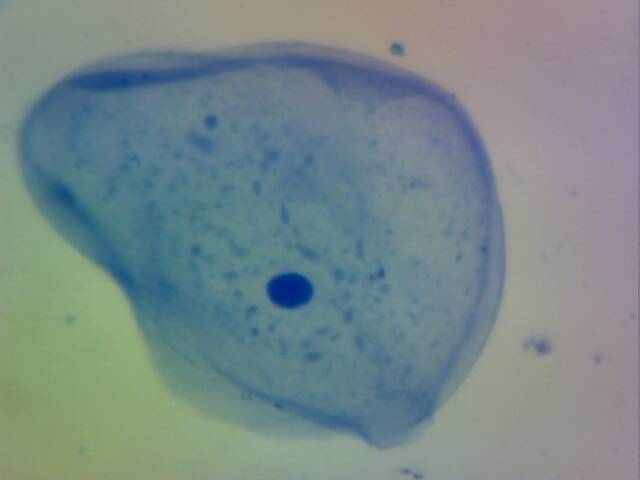
\includegraphics[width=\textwidth]{cheek_cell}
\end{column}
\begin{column}{0.07\textwidth}

\includegraphics[width=\textwidth]{arrow}
\end{column}
\begin{column}{0.27\textwidth}
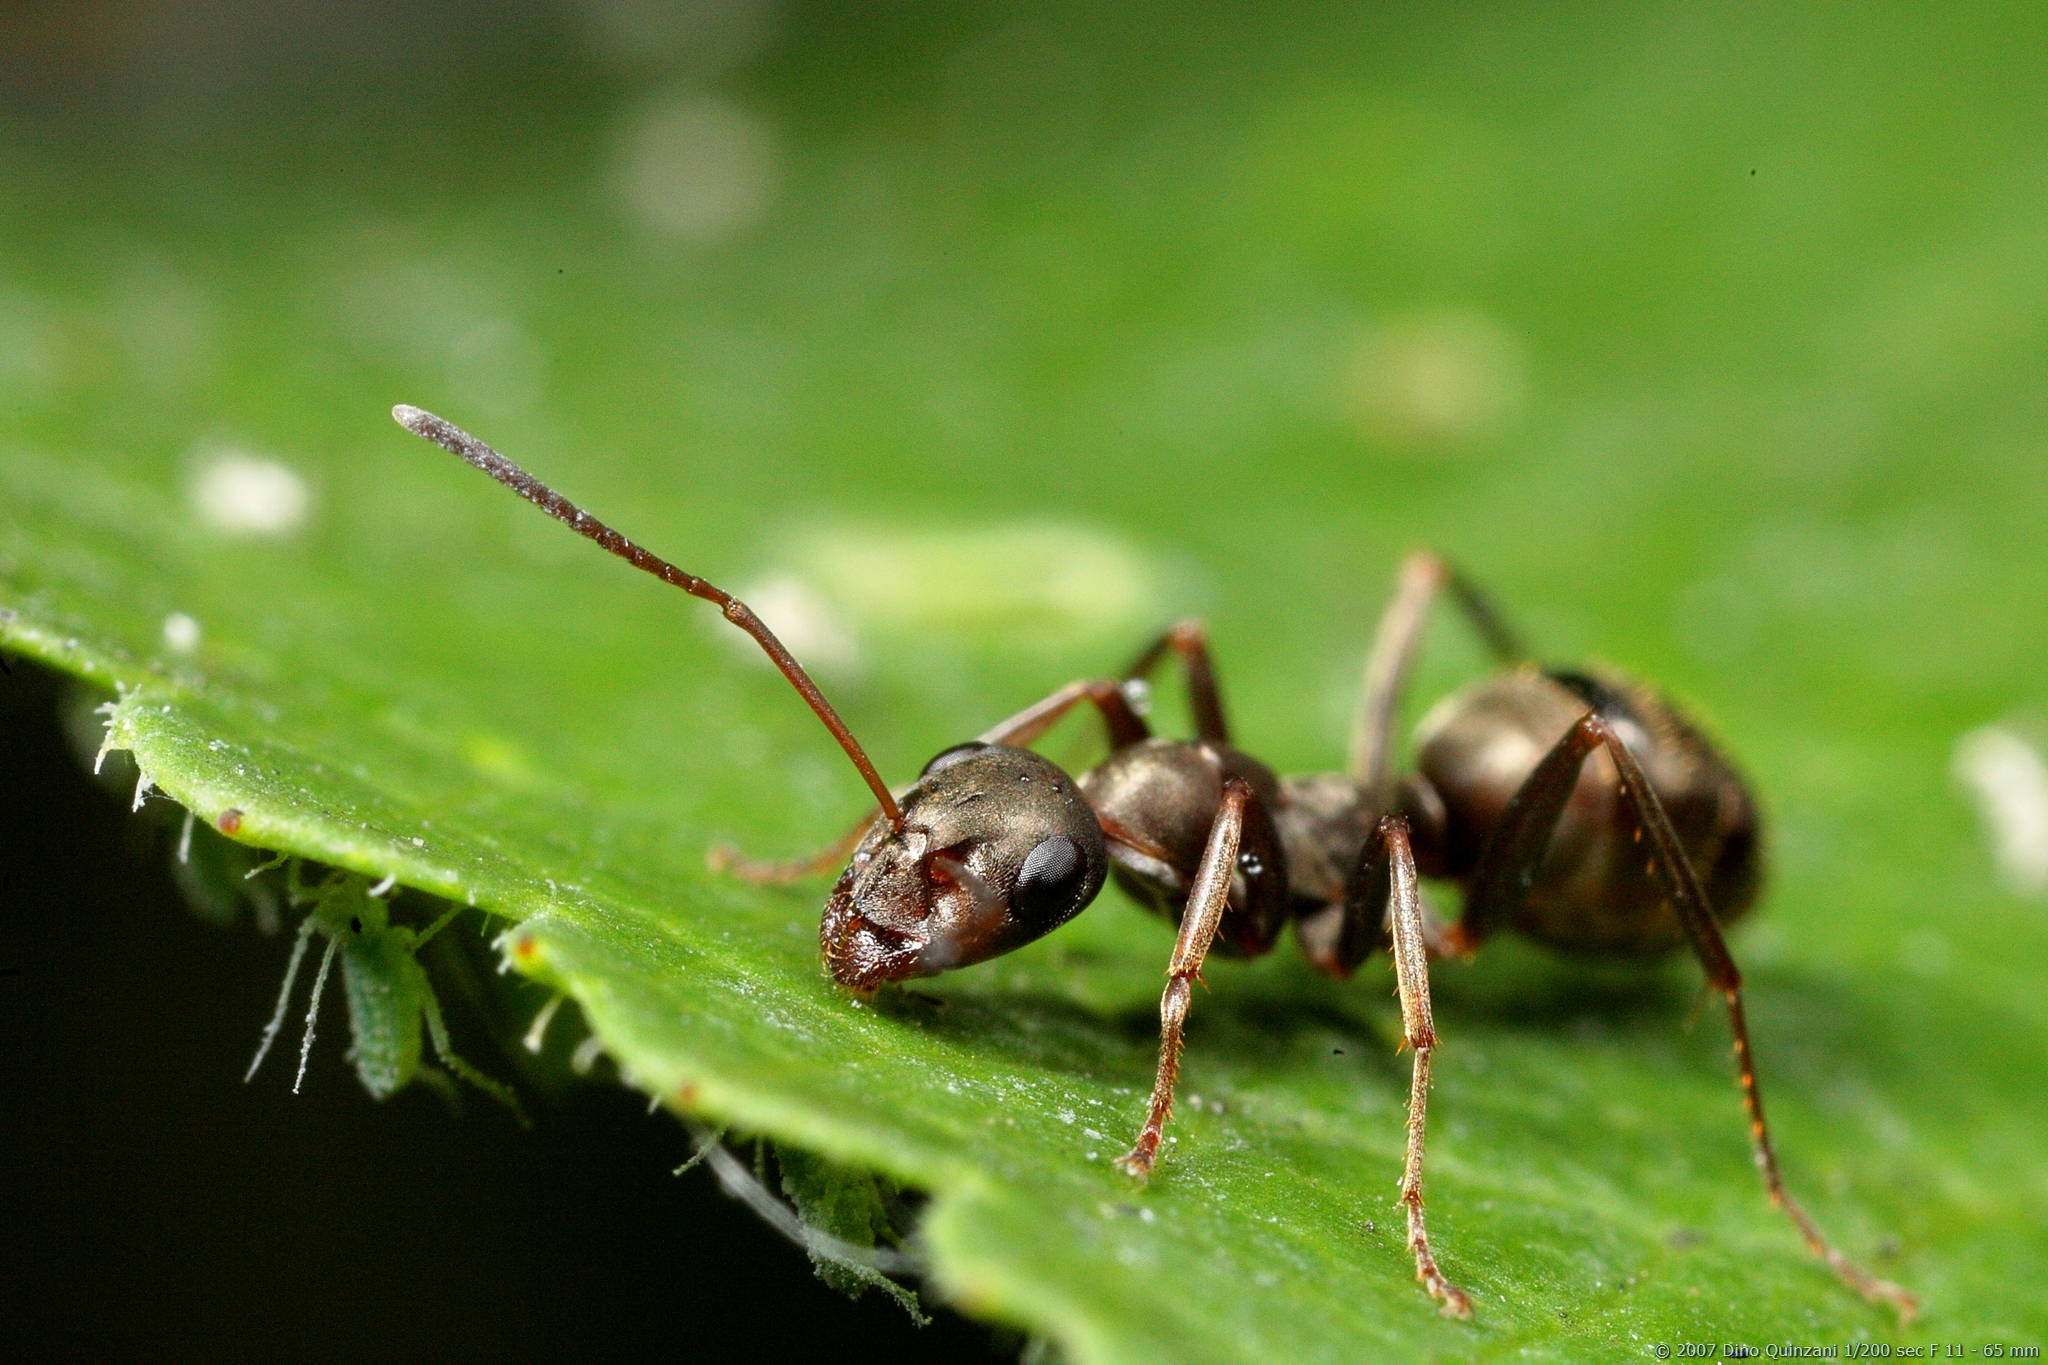
\includegraphics[width=\textwidth]{ant}
\end{column}
\end{columns}
\vspace{1ex}
\begin{columns}
\begin{column}{0.05\textwidth}
\end{column}
\begin{column}{0.27\textwidth}
\centering
cell {\tiny\cite{clare_and_ben_2017}}
\end{column}
\begin{column}{0.07\textwidth}
\end{column}
\begin{column}{0.27\textwidth}
\centering
ant {\tiny\cite{quinzani_2008}}
\end{column}
\end{columns}
\vspace{2ex}
\begin{columns}
\begin{column}{0.05\textwidth}
\begin{subfigure}[b]{\textwidth}
\caption{}
\label{fig:simulated}
\end{subfigure}
\end{column}
\begin{column}{0.27\textwidth}

\includegraphics[width=\textwidth]{cell}
\end{column}
\begin{column}{0.07\textwidth}
{\Large
\includegraphics[width=\textwidth]{arrow}}
\end{column}
\begin{column}{0.27\textwidth}

\includegraphics[width=\textwidth]{clump}
\end{column}
\end{columns}
\vspace{1ex}
\begin{columns}
\begin{column}{0.05\textwidth}
\end{column}
\begin{column}{0.27\textwidth}
\centering
cell
\end{column}
\begin{column}{0.07\textwidth}
\end{column}
\begin{column}{0.27\textwidth}
\centering
clump
\end{column}
\end{columns}
\vspace{2ex}
\caption{Analogy between (\subref{fig:natural}) natural and (\subref{fig:simulated}) simulated hierarchical fraternal transitions of individuality.}

\end{figure}

\end{alertblock}

\begin{alertblock}{Previous Work}
\vspace{1ex}
evolution of digital cell groups with:
\begin{itemize}
\item resource sharing
\item reproductive division of labor
\item reproductive bottleneck
\item apoptosis response to mutation
\end{itemize}

\begin{figure}%[!htbp]
\begin{center}

\begin{subfigure}[b]{0.33\columnwidth}
  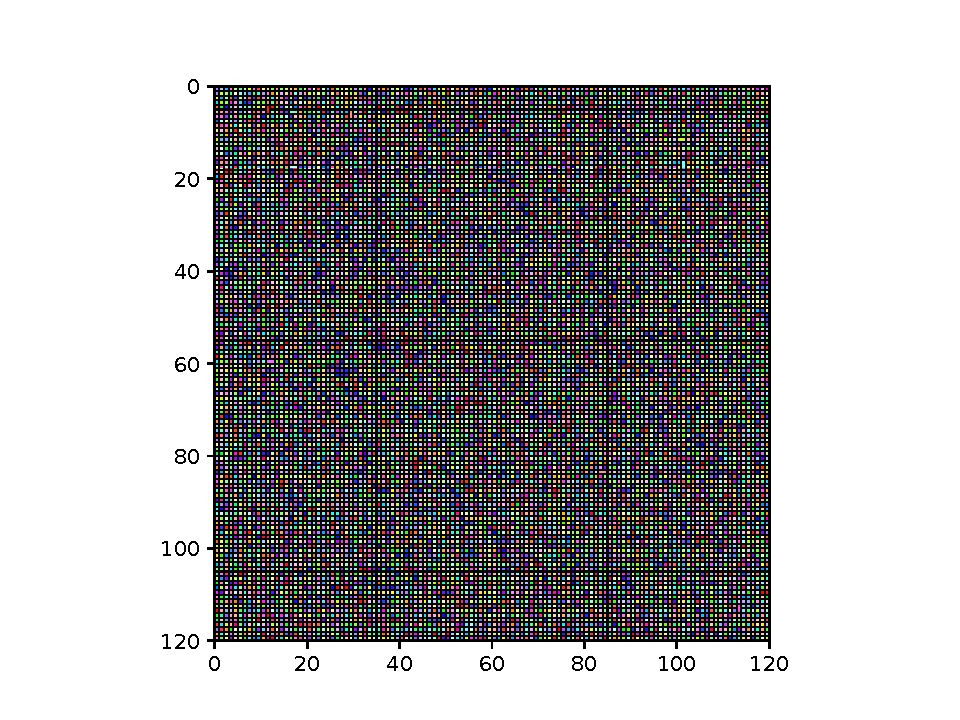
\includegraphics[width=\columnwidth,trim={2.5cm 0.5cm 2.5cm 1cm},clip]{img/ChannelMap_1007_update0}
  \vspace{-5ex}
  \caption{Update 0; cell gen. 0}
  \label{fig:ChannelMap_1007_update0}
\end{subfigure}%
\begin{subfigure}[b]{0.33\columnwidth}
  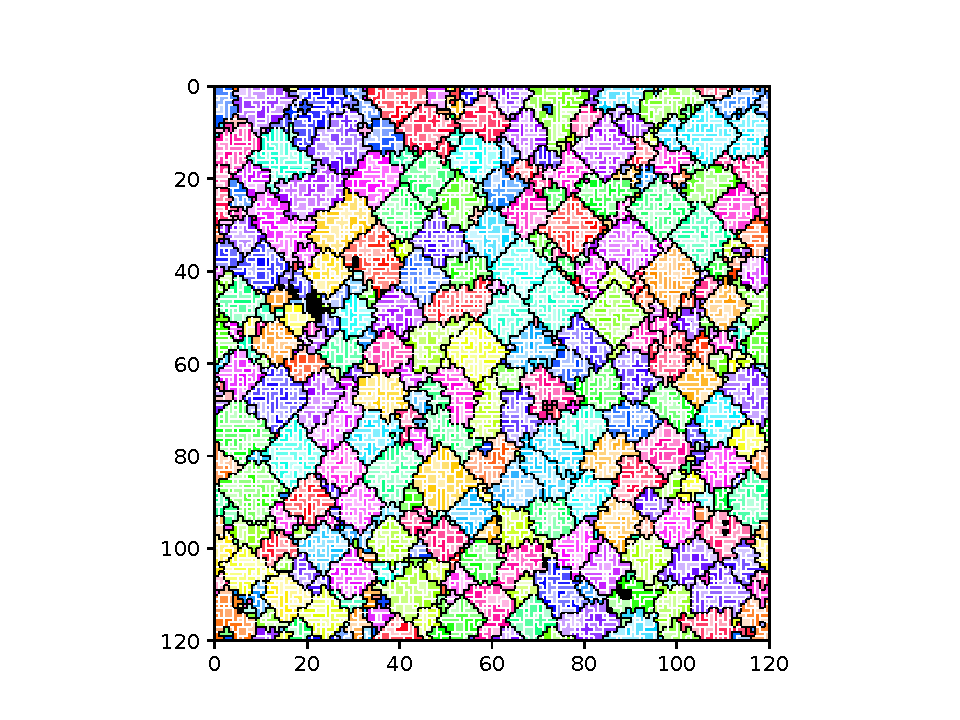
\includegraphics[width=\columnwidth,trim={2.5cm 0.5cm 2.5cm 1cm},clip]{img/ChannelMap_1007_update55520}
  \vspace{-5ex}
  \caption{Update 55520; cell gen. 103}
  \label{fig:ChannelMap_1007_update55520}
\end{subfigure}%
\begin{subfigure}[b]{0.33\columnwidth}
  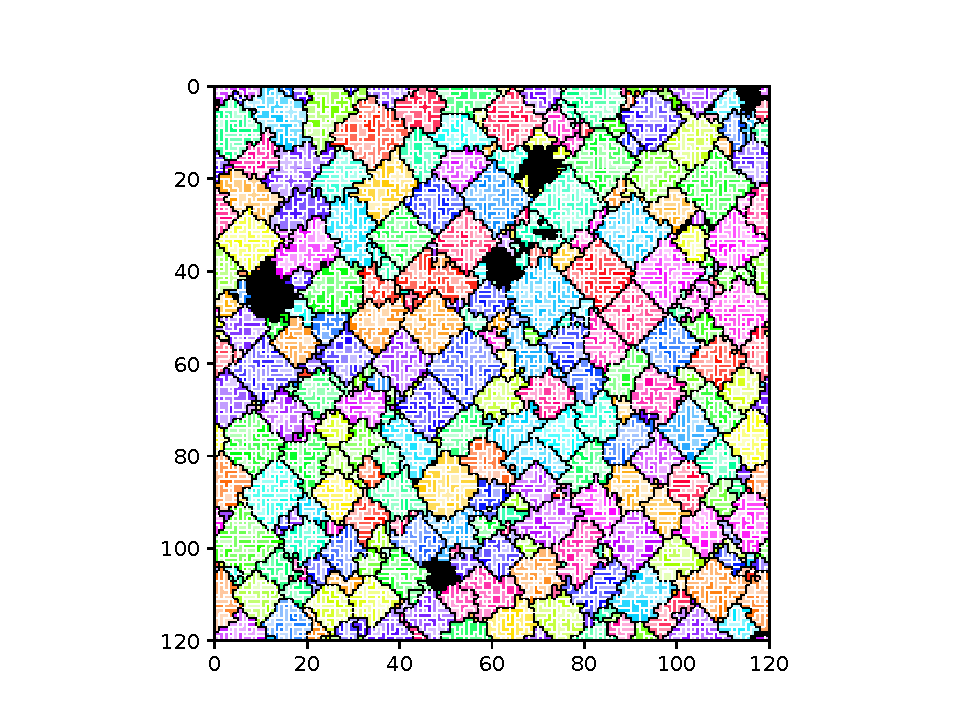
\includegraphics[width=\columnwidth,trim={2.5cm 0.5cm 2.5cm 1cm},clip]{img/ChannelMap_1007_update277600}
  \vspace{-5ex}
  \caption{Update 277600; cell gen. 563}
  \label{fig:ChannelMap_1007_update277600}
\end{subfigure}%

\begin{subfigure}[b]{0.33\columnwidth}
  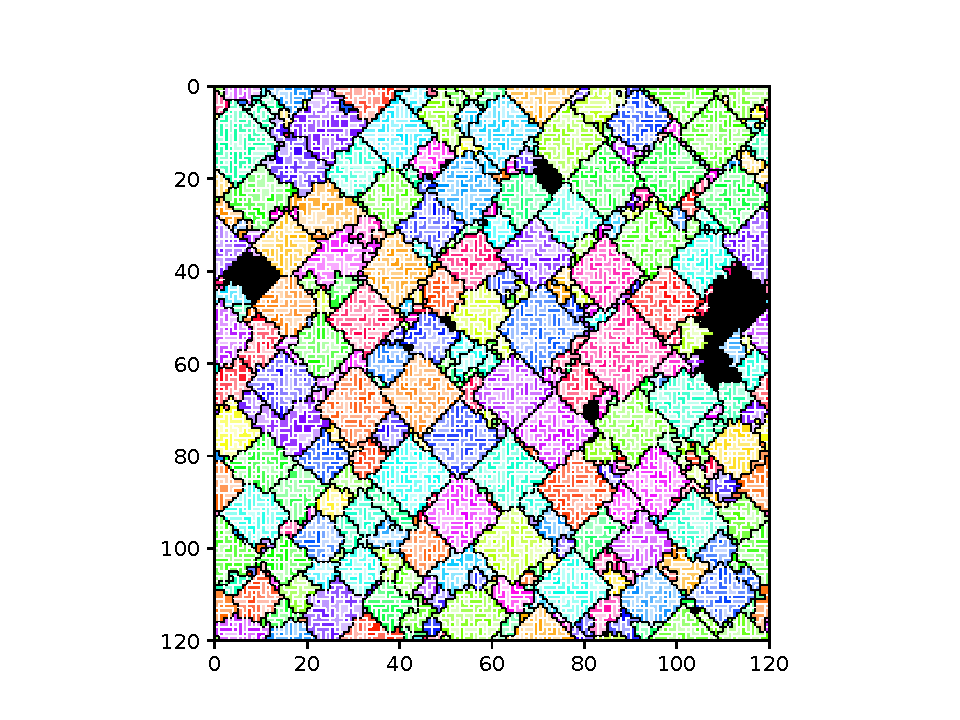
\includegraphics[width=\columnwidth,trim={2.5cm 0.5cm 2.5cm 1cm},clip]{img/ChannelMap_1007_update500000}
  \vspace{-5ex}
  \caption{Update 500000; cell gen. 1072}
  \label{fig:ChannelMap_1007_update500000}
\end{subfigure}%
\begin{subfigure}[b]{0.33\columnwidth}
  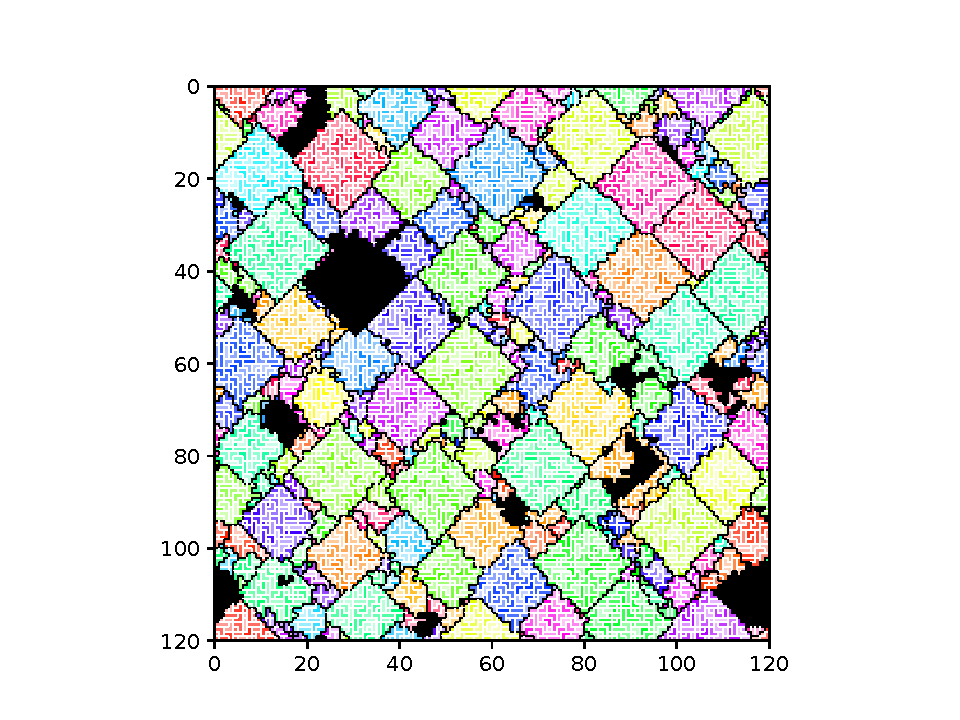
\includegraphics[width=\columnwidth,trim={2.5cm 0.5cm 2.5cm 1cm},clip]{img/ChannelMap_1007_update1000000}
  \vspace{-5ex}
  \caption{Update 1000000; cell gen. 2405}
  \label{fig:ChannelMap_1007_update1000000}
\end{subfigure}%
\begin{subfigure}[b]{0.33\columnwidth}
  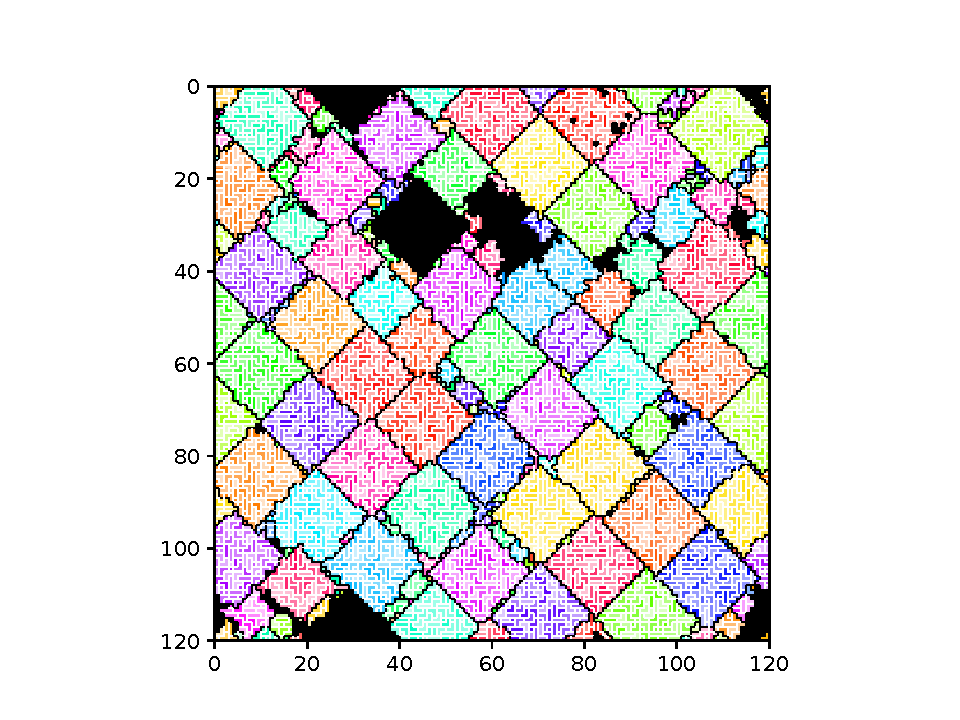
\includegraphics[width=\columnwidth,trim={2.5cm 0.5cm 2.5cm 1cm},clip]{img/ChannelMap_1007_update2000000}
  \vspace{-5ex}
  \caption{Update 2000000; cell gen. 4974}
  \label{fig:ChannelMap_1007_update2000000}
\end{subfigure}

\caption{
Progression of of same-channel level-one and level-two signaling networks states in an evolutionary run where level-two resource sharing evolved.
Level-one channels are coded by color saturation and level-two channels are coded by color hue.
A single cell-like organism occupies each grid tile except for black tiles, which are empty.
}
\label{fig:grid_progression}
\end{center}
\end{figure}


\end{alertblock}


\end{block}


\begin{block}{Acknowledgement}
{\footnotesize
Thank you to CMSE 822 instructor Dr. Sean Couch and teaching assistant Forrest Glines.
This research was supported in part by NSF grants DEB-1655715
and DBI-0939454.
Any opinions, findings, and conclusions or recommendations expressed in this
material are those of the author(s) and do not necessarily reflect the views of the National Science Foundation.\par
}
\end{block}



%------------------------------------------------

%----------------------------------------------------------------------------------------
%	OBJECTIVES
%----------------------------------------------------------------------------------------


%----------------------------------------------------------------------------------------

\end{column} % End of the first column

\begin{column}{\sepwid}\end{column} % Empty spacer column

\begin{column}{\twocolwid} % Begin a column which is two columns wide (column 2)

%----------------------------------------------------------------------------------------
%	IMPORTANT RESULT
%----------------------------------------------------------------------------------------

\begin{block}{Resource Distribution Model}
\begin{figure}[t]
\begin{center}
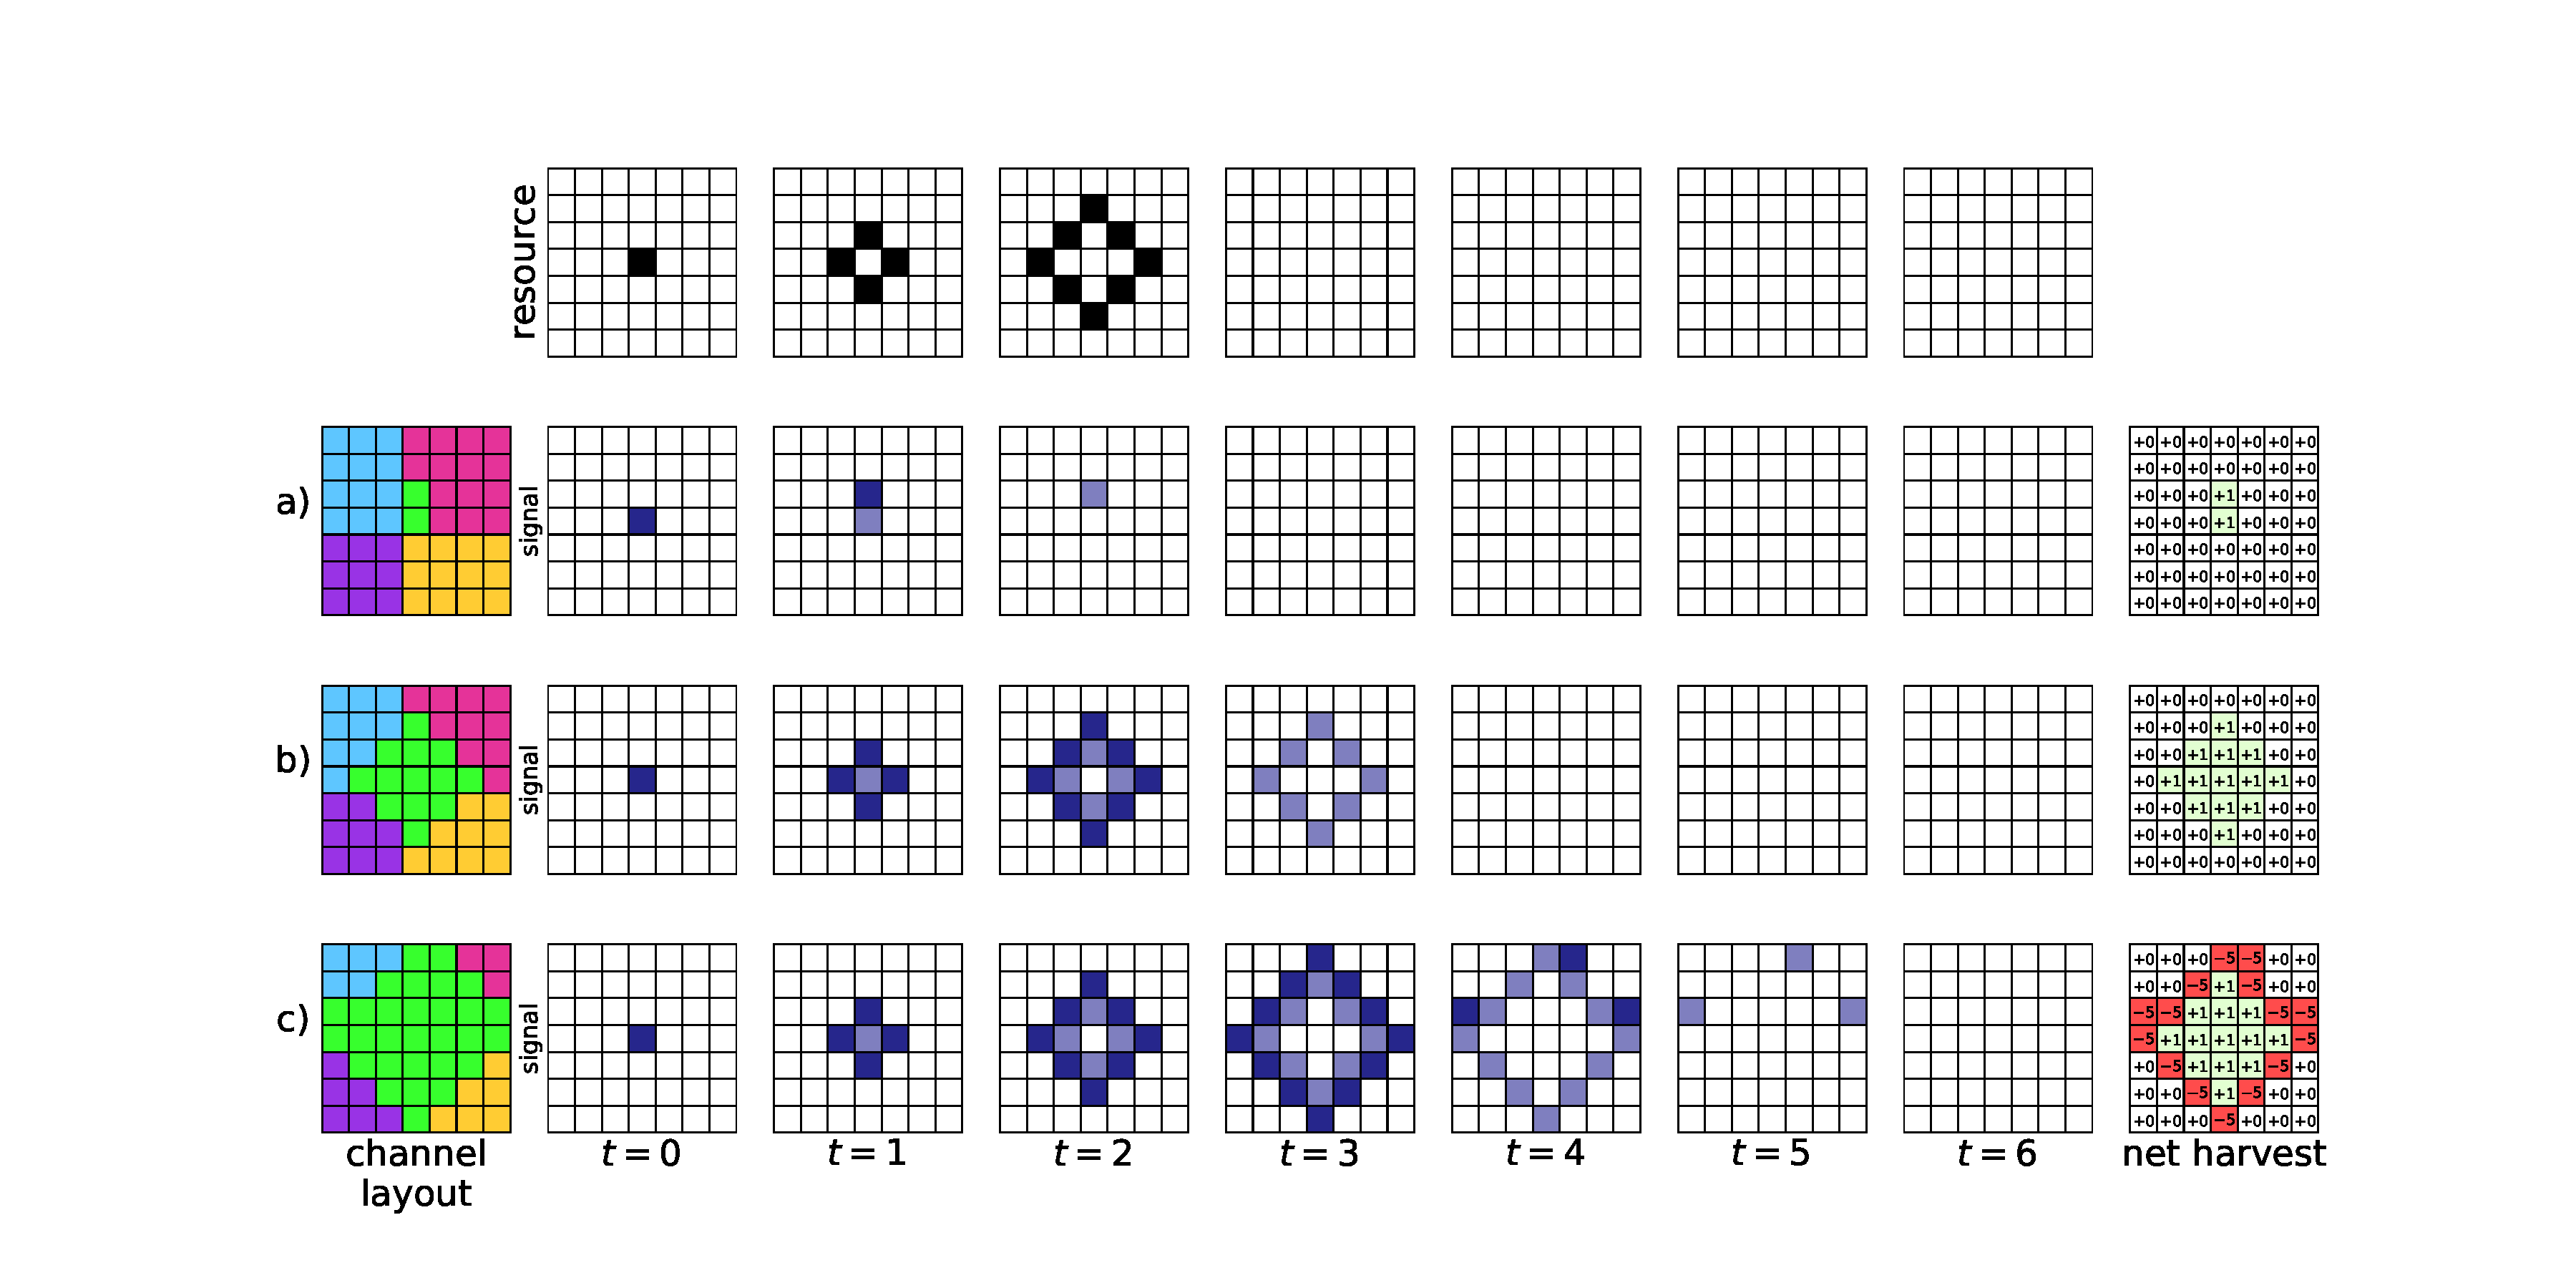
\includegraphics[width=\columnwidth,trim={4cm 0.5cm 4cm 0.5cm},clip]{img/explanatory}
\caption{
\textbf{Activation signaling, and net resource collection for three different-sized same-channel networks during a resource wave event.}
At the top, a resource wave is depicted propagating over three updates and then ceasing for four updates (left to right).
In row $a$, a small two-cell channel-signaling group (far left, in green) is activated; tracking the resource wave (top) yields a small net resource harvest (far right).
In row $b$, an intermediate-sized 13-cell channel-signaling group yields a high net resource harvest.
Finally, in row $c$, a large 29-cell channel-signaling group incurs a net negative resource harvest.
In rows $a$, $b$, and $c$, dark purple indicates the active state, light purple indicates the quiescent state, and white indicates the ready state.
}
\label{fig:explanatory}
\end{center}
\end{figure}

\end{block}



\begin{block}{Strong Scaling}
\begin{columns}
  \begin{column}{0.5\textwidth}
\begin{alertblock}{\textbf{MPI}}
\begin{figure}
    \centering
    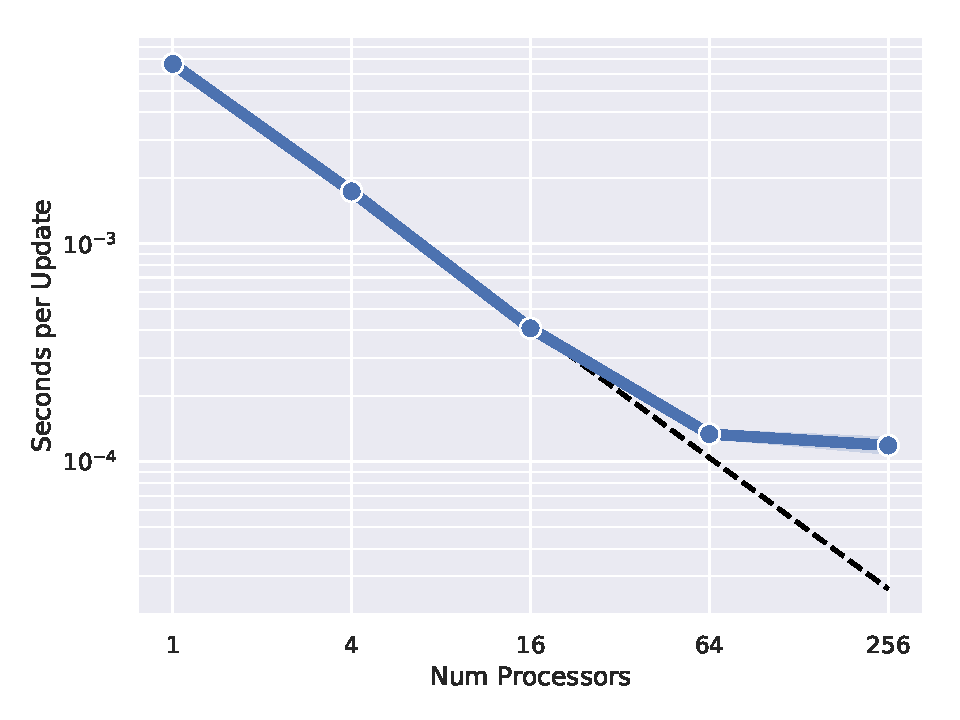
\includegraphics[width=\textwidth]{img/MPIStrong}
  	\caption{
    MPI implementation time to solution versus parallelism for a fixed problem size (a $2048\times2048$ grid).
    Dashed line indicates the ideal scaling relationship.
    Shaded area represents standard deviation of five replications for each observation.
    }
\end{figure}
\end{alertblock}
\end{column}
\begin{column}{0.5\textwidth}
\begin{alertblock}{\textbf{Charm++}}
\begin{figure}
    \centering
    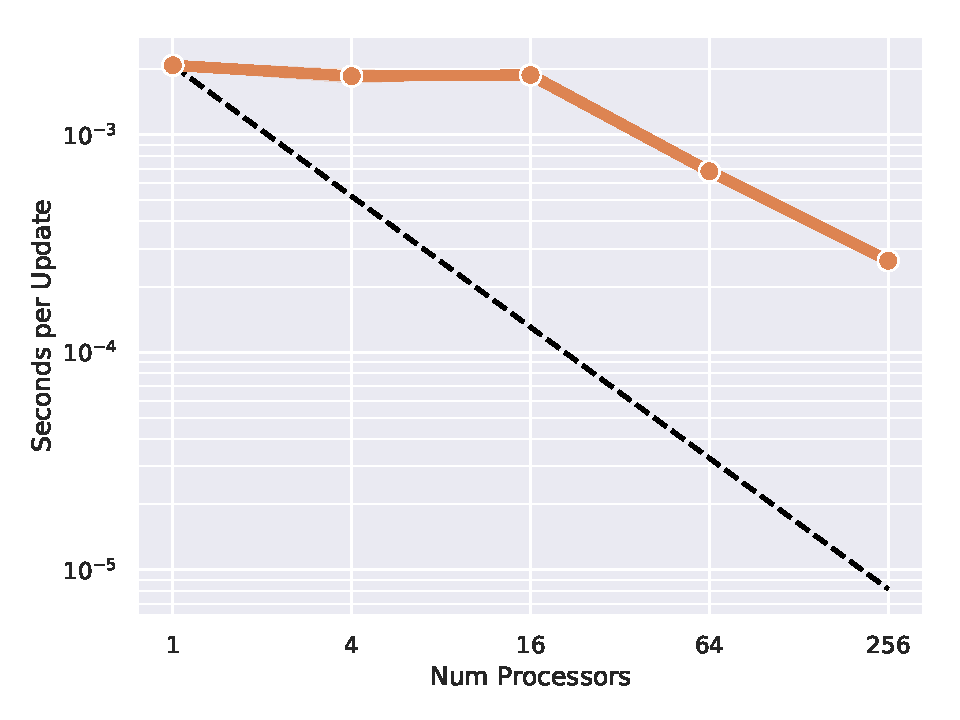
\includegraphics[width=\textwidth]{img/CharmStrong}
  	\caption{
      Charm++ implementation time to solution versus parallelism for a fixed problem size (a $16\times16$ grid).
      Dashed line denotes the ideal scaling relationship.
      Shaded area represents standard deviation of five replications for each observation.
    }
\end{figure}
\end{alertblock}
\end{column}
\end{columns}
\end{block}

\vspace{5ex}


%----------------------------------------------------------------------------------------
\vspace{-6ex}
\begin{columns}[t,totalwidth=\twocolwid] % Split up the two columns wide column again

\begin{column}{\onecolwid} % The first column within column 2 (column 2.1)


%----------------------------------------------------------------------------------------

\end{column} % End of column 2.1

\begin{column}{\onecolwid} % The second column within column 2 (column 2.2)


\end{column} % End of column 2.2

\end{columns} % End of the split of column 2

\end{column} % End of the second column

\begin{column}{\sepwid}\end{column} % Empty spacer column

\begin{column}{\onecolwid} % The third column

\begin{block}{Weak Scaling}
  \vspace{-0.5ex}
\begin{alertblock}{\textbf{MPI}}
\begin{figure}
    \centering
    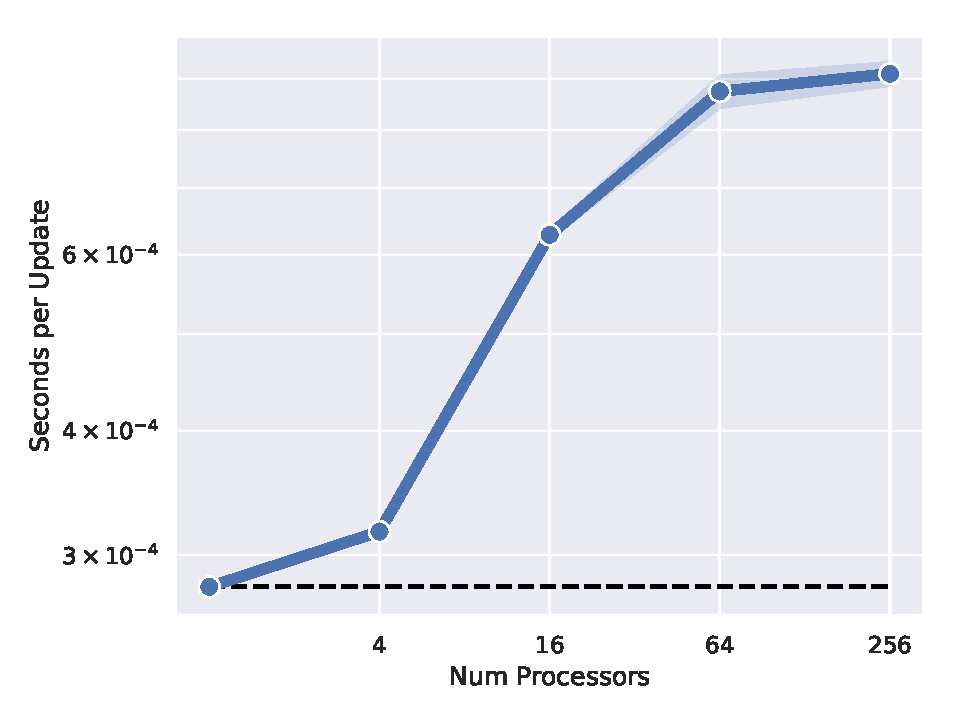
\includegraphics[width=0.9\textwidth]{img/MPIWeak}
  	\caption{
    Charm++ implementation time to solution versus parallelism for problem size proportional to CPU count (262,144 grid tiles per CPU).
    Dashed line indicates the ideal scaling relationship.
    Shaded area represents standard deviation of five replications for each observation.
    }
\end{figure}
\end{alertblock}
\vspace{-0.5ex}
\begin{alertblock}{\textbf{Charm++}}
\begin{figure}
    \centering
    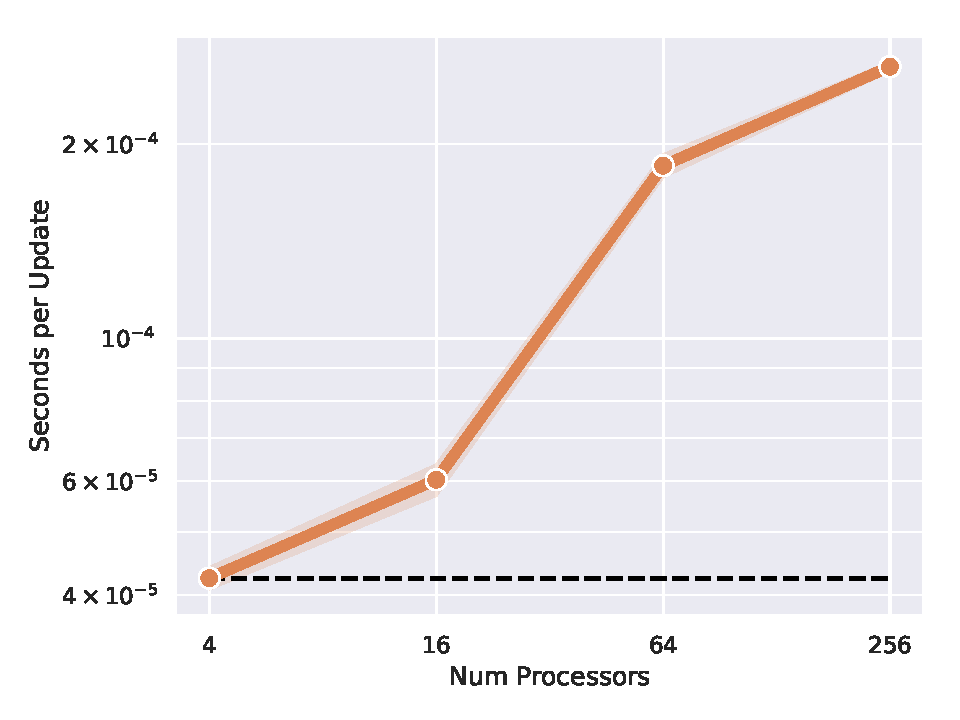
\includegraphics[width=\textwidth]{img/CharmWeak}
  	\caption{
    Charm++ implementation time to solution versus parallelism for problem size proportional to CPU count (1 grid tile per CPU).
    Dashed line indicates the ideal scaling relationship.
    Shaded area represents standard deviation of five replications for each observation.
    }
\end{figure}
\end{alertblock}

\end{block}


\vspace{-0.5ex}
\begin{block}{Discussion}
{\small
\vspace{-1ex}
\begin{itemize}
\item \textit{Charm++ strong scaling:} poor performance when Chares overload available CPUs
\item \textit{MPI strong scaling:} near-ideal only down to a grid chunk size of around $256\times256$, perhaps due to breakdown of latency hiding
\item \textit{weak scaling:} both implementations take a performance hit moving from single- to multi-node
\end{itemize}
}
\end{block}


\end{column} % End of the third column

\end{columns} % End of all the columns in the poster

\end{frame} % End of the enclosing frame

\end{document}
